\chapter{Design Principles of Software-defined Storage}
\label{chap:design_principles}

In this chapter, we describe the design principles for wide-area
software-defined storage.  Our focus is on supporting domain-specific storage
needs for applications that span multiple, changing
organizational domains.  We describe our high-level design requirements,
and flesh out an SDS system specification in terms of its data plane, its
control plane, and its view changes.

\section{Overview}

The design principles for software-defined wide-area storage are rooted in 
our observations of three ``tussle spaces''~\cite{david-clark-tussle-spaces}.
These are (1) the physical storage substrate that hosts and serves the raw
bytes, (2) the applications' domain-specific storage requirements, and (3) the trust
relationships between the users and organizations who interact with shared
data.

The goal of SDS is to allow application developers and users to efficiently accomodate tussles
in all three of these domains simultaneously.  Prior work in this space
only accomodates at most two tussles (Chapter~\ref{chap:related-work}).

\subsection{Challenges}

Designing applications to be portable across services helps address tussles in
storage services and tussles in application storage semantics.
However, the cost of porting $m$ applications to $n$ services
today requires $O(mn)$ patches.  This is true even if developers share their
patches---getting a patch to work with one application can require completely
re-writing it to work with another application.

We do not believe this patch situation will improve on its own,
since developers are incentivized to ship code that \emph{works
today} as opposed to code that is portable to unspecified systems at unspecified
times in the future.  Moreover, the business models of commodity cloud services
depend on customers continuously paying for the service, and are thus
disincentivised to help make applications portable to their competitors.
Even if portability was a desireable and achievable design goal from the get-go,
getting $m$ applications to adopt a new service's behavior would still at best
require $O(m)$ man-hours.

Designing applications to accomodate tussles in trust relationships has been
addressed today through federations and open-membership systems.
In federations, each organization promises to adhere to a
``common ground'' data-hosting policy that allows them to interoperate, so that
users that trust one organization in the federation can trust other
organizations (and similarly, one organization can trust another organization's
users).  For example, the operators of a set of organizations may agree to use an agreed-upon
single-sign-on (SSO) system to authorize computers from different organizations
to access sensitive data.  As another example, a set of organizations may agree
to use a common data format and API for sharing data with one another (such as
putting their data servers behind an API endpoint that emulates Amazon S3).

The trouble with federations is that they impose a high coordination overhead on
the participating organizations.  Organization administrators must regularly
communicate and coordinate to adapt to changing services and organization
boundaries.  This imposes a high standing cost on participating in the
federation, which can be too burdensome for marginalized players.  For example,
federations governed by in-person meetings exclude individuals who cannot
travel easily.  As another example, federations whose coordination occurs in English
penalizes non-English-speaking participants.  As a third example, organizational
representatives can advocate for the use of legally-encumbered (e.g. patented)
services and technology that is not available in all jurisdictions, or only
available at non-trivial cost to the organizations' users.

Open-membership systems attempt to address the limits of federation by embedding
all inter-organization coordination in the protocol itself.  The rationale is
that this reduces the need for organization administrators to coordinate in
order to run the system.  In the vernacular, these systems are often referred to
as ``trustless'' systems because the user does not need to place trust in any
governance mechanisms for the application to work.  Examples include peer-to-peer file sharing
(like BitTorrent~\cite{bittorrent} and Vanish~\cite{vanish}) and cryptocurrencies (like
Bitcoin~\cite{bitcoin} and Ethereum~\cite{ethereum}).

The difficulty with designing open-membership applications is that they cannot
be upgraded easily.  The lack of out-of-band coordination between organization
administrators means that developers forgo the ability to change the protocol
once deployed.  Attempting to introduce a backwards-incompatible change to the
application is tatamount to creating a whole new application.  For example,
the Bitcoin Cash network~\cite{bcash} split off from the Bitcoin network 
due to a disagreement in the system's maximum throughput (a one-line code
change).

\subsection{Objectives}

The physical storage substrate includes the existing cloud services that can be
reused to host and serve data.  Moreover, this includes any \emph{future}
storage services that may be developed after the application is build and
deployed.  We want the developer to be able to use any existing systems
they want, while preserving low switching costs.  This leads to our first
objective:
\\
\\
\noindent{\textbf{Objective 1}}: \emph{Once developed, an application must be able to use any future storage
system to host data without changing its storage semantics.}
\\
\\
At the same time, the set of applications using a given storage system may
undergo changes that make them incompatible with its semantics.  For example,
the application developer may discover that the users require stronger
consistency guarantees than the storage system can offer.  The developer cannot
simply move to a different system on a whim, since all of the data is hosted 
on the current system.  At the same time, the developer cannot be expected
to rewrite the application to keep using it.  This leads to our second
objective:
\\
\\
\noindent{\textbf{Objective 2}}: \emph{Once chosen to host data, a storage system must remain compatible with any
future changes to an application's storage semantics.}
\\
\\
All the while, the trust relationships between users and organizations have
an effect on how applications are permitted to interact with their data.
The trust relationships between users ultimately govern how they can interact
with each other's data.

For example, a corporate manager may use an SDS system to give her employees access
to confidential company records only during business hours, and only from 
within a whitelist of company-approved networks.
As another example, an serial movelist may use SDS to
make a new ebook chapter readable only to users who pay her at first, but then release it
to the public after a certain amount of time has passed.  As a third example,
a user group in an online public forum may use SDS to filter the data they read,
such that abusive users' content is automatically discarded.

In order to handle these application requirements, we must meet a third
objective:
\\
\\
\noindent{\textbf{Objective 3}}: \emph{Users must be able to bootstrap trust in one another independent of the
applications and the storage systems they use.}
\\
\\
If we can do this, then it becomes possible for users and organizations to
identify with whom they will share data, as well as describe non-trivial
policies governing that sharing (i.e. policies beyond ``share with no one'' or ``share
with the whole world'').  They do not need the application developer to be aware
of the user's trust relationships, nor do they need the developer to attempt to
provide tools to address them.  This is a departure from multi-user Web
applications today, for example, which often provide their own user interfaces
for managing data sharing.

These policies may not even be known to users when they start using the application, since
discovering that they are needed at all (e.g. the case of filtering
abusive users) requires them to use the application for some time.  Moreover,
the policies must be enforcable across organizational boundaries.
Our final objective, then, is that:
\\
\\
\noindent{\textbf{Objective 4}}: \emph{Users must be able to set data-sharing policies
for their data that are enforced independently of the applications and underlying storage
systems}.
\\
\\
In the remainder of this chapter, we show how to meet these objectives shape
sculpt the design space of SDS systems.  We
conclude by distilling the design space into a set of principles for
software-defined storage design and implementation.

\section{Requirements}

\begin{figure}[h]
   \caption{Logical representation of a wide-area SDS system.  The SDS system
   is a cross-organization intermediate layer that connects services to
   applications via distinct interfaces.}
   \centering
   \includegraphics[width=0.9\textwidth,page=2]{figures/dissertation-figures}
   \label{fig:chap2-sds-overview}
\end{figure}

At a high-level, an SDS system is a logical ``hub'' between applications and
services that spans multiple organizations (Figure~\ref{fig:chap2-sds-overview}). 
The hub takes reads and writes from the application, processes them
according to application-defined semantics, and loads and stores the resulting
data to the underlying storage systems.
It offers two interfaces:  a \emph{service interface} through which it interacts with
services on the applications' behalf, and an \emph{application interface} through
which applications interact with data and define their desired storage
semantics.

\subsection{Service Interface}

The service interface is similar to existing work on service compatibility
libraries.  In particular, the interface allows SDS to divide the set of
services into three distinct classes, where each class has a driver model that
when implemented will enable applications to use it.  The service driver models
enable the following:

\begin{itemize}
   \item \textbf{Treat cloud storage as disk}.  The set of cloud storage
      services in use must collectively appear to be a single
      read/write storage medium with a uniform access interface.
   \item \textbf{Treat data sets as read-only disk}.  The set of individual
      data sets in use must collectively appear to be a single read-only
      storage medium with a uniform access interface.
   \item \textbf{Treat CDNs as a write-through cache}.  The set of CDNs used by an
      application must \emph{not} affect the end-to-end consistency model, even if the
      CDN is misconfigured or maliciously serves stale data.  SDS must make CDNs
      appear to be write-coherent caches that only improve read performance.
\end{itemize}


\begin{figure}[h]
   \caption{Service and aggregation drivers in an SDS system.  Aggregation
   drivers span multiple organizations and route application reads and writes to
   one or more service drivers.}
   \centering
   \includegraphics[width=0.9\textwidth,page=3]{figures/dissertation-figures}
   \label{fig:chap2-driver-overview}
\end{figure}

Logically speaking, service drivers run at the service-facing ``bottom'' of the
SDS ``hub'' (Figure~\ref{fig:chap2-driver-overview}).
They handle only the data meant to be hosted on the service.  The SDS system may
instantiate multiple copies of the service drivers in order to handle higher
load or keep applications isolated from one another.

\subsection{Application Interface}

Developers need to be able to specify
end-to-end storage semantics across an aggregation of services
in a multi-user setting.  To enable this,
SDS offers a separate type of driver model called an ``aggregation
driver.''

There is one aggregation driver per application.  Logically speaking, it runs at
the ``top'' of the SDS ``hub'' (Figure~\ref{fig:chap2-driver-overview})
and mediates all requests between users and
service drivers (for the duration of this thesis, we will not
distinguish between users and the application clients
they run).  It mediates interactions in terms of \emph{which user} issues the
interaction, \emph{which operation} is requested, \emph{which data
record} is affected, and \emph{which network host} is originating the request.

The high-level idea behind having two driver classes is that once a service has an appropriate service driver,
it can be ``plugged into'' the SDS system such that existing aggregation drivers
can use it immediately.  An aggregation driver implements the application's desired end-to-end storage
semantics, and translates
application-level requests into requests understood by the service driver.  These
requests are issued such that their execution
by service drivers delivers the desired end-to-end behavior.  This reframes the
costs of porting applications to services:

\begin{itemize}
    \item For the cost of writing only the application-specific
aggregation drivers, a new application can be made
compatible with all existing and future services with no modification.
    \item For the cost of writing only the service-specific SDS driver, a new
service can be made compatible with all existing and future applications.
\end{itemize}

In other words, the cost of porting $m$ applications to $n$ services can be
reduced from $O(mn)$ to $O(m+n)$.
To realize this cost savings, many applications will share an SDS system.  Aggregation and service drivers
will be \emph{decoupled} from the applications---they will be
developed independently of one another, and independently of the
application itself.

\subsection{Data and Control Planes}

The primary task of the SDS system is to move data from users to services and from
services to users.  However, it needs to move each user's data
subject to the application's specific storage semantics.

To address these two requirements, we formulate SDS in terms a
data plane and a control plane.  The \emph{data plane}'s job
is to ensure all-to-all connectivity between users and service processes.
It moves the raw bytes between services and users, but with no concern for
application-specific semantics.  It includes the service-facing interface, the
service drivers, and the data formatting, serialization, routing, and transmission
logic.

The \emph{control plane} implements each application's
storage semantics by acting as a governor for the data plane.
It runs an application's aggregation driver 
to constrain how each of its users interact with the data plane.

The data plane is shared by all applications and all services, and implements a
common data-sharing interface via a fully-connected bidirectional communication graph.
Every node in an SDS-powered application can send and receive data-plane
messages to every other node.  The control-plane defines the behavior of the
system insofar as what messages get sent in reaction to I/O, and how they are
transformed before being routed to and from the underlying services.

\section{Data Plane}

The SDS data plane organizes data into units called \emph{chunks}.  Chunks form
the basis of all data within SDS, and constitute a ``narrow waist'' between 
a multitude of service drivers below and a multitude of aggregation drivers
above.  Chunks have the following properties in SDS:

\begin{itemize}
    \item Every piece of data in SDS is made of one or more chunks.
    \item Each chunk is immutable.
    \item Each chunk has a globally-unique identifier.
\end{itemize}

The data plane ensures that each chunk belonging to a particular application
is addressable (but not necessarily resolvable) by every process connected to it.
If the control plane logic allows it, each application
process can resolve and download chunks created by other processes in the same
application.

\begin{figure}[h]
   \caption{The narrow waist in the SDS data plane.  The aggregation driver
   translates application-level storage requests into operations on manifests
   and chunks, and service drivers implement simple \textit{create},
   \textit{update}, and \textit{delete} operations on chunks using existing
   service interfaces.}
   \centering
   \includegraphics[width=0.9\textwidth,page=4]{figures/dissertation-figures}
   \label{fig:chap2-narrow-waist}
\end{figure}

At the service driver level, the SDS
system provides operations to \texttt{create}, \texttt{read}, and
\texttt{delete} chunks.  Service drivers execute the requisite protocols
and data transformations to
marshal chunks back and forth to their respective services.

At a layer above the service drivers but beneath aggregation drivers, SDS
groups chunks that belong to the same piece of application data using two specialied
chunk types:  a \emph{block} and a \emph{manifest}.  A block is simply a data
container with a known length.  A manifest identifies a sequence of blocks.
They constitute the ``narrow waist'' of an SDS system's data plane
(Figure~\ref{fig:chap2-narrow-waist}).

Blocks and manifests provide just enough information to allow us to define a
set of generic operations for manipulating application data, but
without mandating a particular data representation or access interface.
Specifically, they allow us to define data-plane operations on
application data in terms of the chunks that make them up:

\begin{itemize}
   \item \textbf{Reading data}.  To read a piece of application data, an SDS client locates
    its manifest, fetches it, and then fetches the blocks listed within it.

   \item \textbf{Creating data}.  To write a new piece of data, an SDS client replicates
    its set of chunks and a manifest that contains them.

   \item \textbf{Updating data}.  Modifying an existing
    piece of application data is done by creating blocks with the modified data,
    creating a new manifest with the ``latest'' sequence of blocks, and deleting
    blocks that contain overwritten data.

   \item \textbf{Deleting data}.  Deleting the data is done by
    deleting its manifest and blocks.
\end{itemize}

These operations are what allow us to implement end-to-end
guarantees with higher-level aggregation drivers without having to interface
directly with services.  SDS client libraries translate application-level data
operations into one or more of these operations.

A key advantage of this protocol is that it gives service drivers insight as to whether or not a
chunk is a block or a manifest, as well as insight on which application-level
datum is being processed.  We exploit this in practice to implement
service drivers to transparently carry out both chunk-level and application
data-level optimizations like de-duplication, compression, batch-writes,
defragmentation, and so on.

\subsection{Data Discovery and Indexing}

Ensuring that chunks are globally-addressable requires maintaining a global
chunk inventory so other processes can discover them.  Any time a user creates,
updates, or deletes data, it creates a new manifest
with a new globally-unique identifier.  In order to read the data, a reader
needs to discover the new manifest identifier and the set of SDS-connected
processes that can serve it.  This responsibility is fulfilled by a data plane
subsystem called the metadata service.

\begin{figure}[h]
   \caption{SDS Metadata Service.  The MS resolves names to their current
   manifests, and allows gateways to update the name/manifest binding.
   Manifests are stored in the underlying storage services, and
   point to the set of blocks that make up the datum.}
   \centering
   \includegraphics[width=0.9\textwidth,page=5]{figures/dissertation-figures}
   \label{fig:chap2-metadata-service}
\end{figure}

The \emph{Metadata Service} (MS) helps users discover the
availability of new chunks, announce the existence of chunks they create, and
identify which SDS-connected processes that can serve a chunk
(Figure~\ref{fig:chap2-metadata-service}).
There is one MS per SDS instance, and
applications share the MS as part of sharing the SDS deployment.

The MS implements an indexing service for manifests.  It binds an unchanging
application-chosen name to a datum's ``latest'' manifest
identifier, and stores the list of SDS-connected processes that can serve it.
Writers set the manifest identifier for a name when they write to the datum.
Readers resolve the datum's identifier to the ``latest'' manifest identifier,
and then proceed to query the MS for the list of processes that can serve its
chunk (i.e. by asking for their network addresses).

\subsubsection{Name Consistency}

The consistency model of the MS's name/identifier mappings determines the \emph{default}
consistency model for an SDS's data.
In our SDS prototype, for example, the MS offers
per-name sequential consistency.  Once a writer successfully updates the manifest
identifier for a name, all subsequent reads on the name will return the new
identifier.

SDS supports different consistency models in part by allowing the
developer-supplied aggregation driver to decide exactly when to update
the manifest identifier as part of an on-going read or write.
This is enabled through the aggregate driver programming model,
described in Section~\ref{sec:aggregation-driver-model}.

\subsubsection{Service Discovery}

In addition to naming manifests, the MS remembers which processes
(i.e. which host/port pairs) are able to serve the manifest and block chunks.
This information is conveyed by the writer when announcing a new manifest,
and given to readers when querying manifests.

The MS also plays a role in deploying service and aggregation drivers.  The
developer uploads new code to the MS, and the MS ensures that the new drivers
are used to service all subsequent read and write requests.  This is described
in detail in Section~\ref{sec:view-changes}.

\section{Control Plane}

An aggregation driver can be thought of as a closure running in the SDS ``hub''
that mediates all interactions with the application's data.  Each aggregation
driver is on the read and write paths for all application processes (including
both users and ``server-side'' processes that run computations over user data).

The control plane's job is to ensure that the application's aggregation
drivers are executed to handle each user's requested data operations.
Designing a suitable control plane and suitable aggregation driver
model is nontrivial and poses several challenges.  These challenges include:

\begin{itemize}
    \item \textbf{Scalability}.  The control plane must be able to service a
    scalable number of concurrent user requests. 
    \item \textbf{Virtualization}.  The application's service and aggregation
    drivers may only interact with its users' data.  Put another way,
      the SDS system must give the application (and all the organizations using
      it) the illusion that it is the sole program using the system.
    \item \textbf{Trusted Computing}.  Since drivers may carry out sensitive,
    data-specific operations (e.g. payment processing, handling proprietary
    data), an organization needs to be able to control which hosts run which
    drivers.  That is, an organization needs to
    control how its users' data gets processed without having to trust or rely
    on other organizations.
    \item \textbf{Driver Agility}.  The control plane must allow an organization to
    change the service and aggregation drivers at run-time.
    This is required in order to fix bugs, improve service, and set policies.
    Organizations must be able to upgrade their drivers independently of other organizations.
    \item \textbf{Fault Tolerance}.  The control plane must be able to identify
    and recover from crashes and slowness from both services and drivers.
\end{itemize}

Addressing scalability requires a \emph{physically distributed control-plane} that can
scale horizontally.  That is, the request volume the system can process must
increase linearly with the number of computers added.
A key design requirement is that aggregation drivers should not become ``accidental
bottlenecks'' simply because they are on all of the applications' users' read/write paths.
Addressing virtualization and trusted computing requires that developers have some
control as to when and where drivers run (i.e. which hosts and users).

\subsection{Volumes}

To address our virtualization requirement, an SDS system
implements a volume abstraction.  A \emph{volume} is a logical grouping of
application data that is available through a fixed set of services and accessed
using the same storage semantics.  That is, data in a volume are loaded and
stored with the same service drivers, and accessed by the application through
the same aggregation driver.  An application has at least one volume, and may have many.

Volumes serve as the SDS storage multiplexing mechanism.
A volume has a designated ``owner'' user that has the power to
change the aggregation driver of a volume on-the-fly, and can add and remove
service driver instances to a volume in order to change where the volume data is
hosted.  In practice, the volume owner user is a privileged
user in the organization.

Each organization manages its own set of volumes.  Organizations implement their
volumes' aggregation drivers to mediate access to the volumes' data,
and use their service drivers to implement
their respective data-hosting policies.

For example, a lab's PI may want a volume that stores data to Amazon S3 and
retains any written data for at least a year for auditing purposes.  The
volume's service driver would be deployed with the read/write credentials to the
PI's S3 bucket, so anyone who can access the volume via the SDS system would indirectly load and
store data to S3.  The PI would deploy an aggregation driver for the volume that
ensured that only other lab scientists could read and write, and ensured
that whenever someone deleted data less than a year old, a hidden copy would be retained
before actually being removed.

As part of addressing SDS data virtualization, the SDS MS assigns each volume 
its own data index state.

\subsection{Gateways}

While we have thus far characterized the SDS control-plane as a ``hub'' that
runs drivers to link services to applications, this is only the \emph{logical} model.
In order to address our control plane design goals, an SDS system must
allow the aggregation driver logic to
span an \emph{arbitrarily large set} of computers and networks.  We introduce
\emph{gateways} as an SDS design element to instantiate and coordinate running
aggregation driver logic.

It is tempting to limit aggregation drivers to
running within a ``centralized'' cluster of application-controlled servers,
such as a set of VMs in a commodity cloud computing service.  Indeed, this is
what most Web applications do today with their data:  all reads and writes are routed through a
central set of servers (e.g. a datacenter) that addresses all of the above
concerns.

This is not an adequate solution for multi-organization applications.
Using application-controlled computing providers for control-plane processing
may violate per-organization data hosting policies.  Each organization using the application
would have to expand its trusted computing base to include the developer-chosen
computing provider.  This breaks our trusted computing requirement, since each
organization must be able to unilaterally set and enforce policies on the data
they produce.  In fact, our sample SDS applications
(Chapter~\ref{chap:applications}) \emph{could not be built to specification} if
developers were not free to control where certain aspects of the storage logic
were executed, since the storage system's correctness depends on it.

Our solution is to distribute the aggregation driver across each organization,
and allow the principal that owns the volume to control which organization runs
which piece of the driver.
What we propose is a programming model that allows the following:

\begin{itemize}
   \item \textbf{Cross-organization modules}.  The driver code
      can be split up into distinct modules that can be
      assigned to different organizations' computers.  This would allow
      developers to keep sensitive code or code for processing sensitive data
      in secure places.
   \item \textbf{Module independence}.  Once written, modules should be reusable in 
      new, different contexts.  This means that the programming model should
      encourage developers to keep modules as independent of one another's
      designs and implementations as possible.
   \item \textbf{Familiar programming}.  The driver programming model
      should not impose any specific programming paradigm on specific modules,
      and it should make it easy for developers to reason about how modules
      interact.
\end{itemize}

We distribute the drivers by way of a set of SDS processes called gateways.
A \emph{gateway} is a control plane process that the
volume owner can program to run part of the aggregation driver code.  The SDS control plane
runs one or more gateways that cooperate to execute drivers in response
to reads and writes (Figure~\ref{fig:chap2-gateways}).

\begin{figure}[h]
   \caption{SDS Gateways.  Gateways coordinate with one another across
   organization boundaries to service read and write requests originating from
   within their organization.  They run a ``stage'' of the volume-wide aggregation driver,
   and run zero or more service drivers instances to load and store chunks to
   service the stage.}
   \centering
   \includegraphics[width=0.9\textwidth,page=6]{figures/dissertation-figures}
   \label{fig:chap2-gateways}
\end{figure}

Gateways present application clients with one of a set of high-level data access
interfaces (like a POSIX filesystem or a SQL database abstraction).
The gateway implementation translates requests to this interface
into data-plane requests for manifests and blocks.

Once the gateway receives the application request, it coordinates with other
gateways in the same volume to service the request in the manner prescribed by
the aggregation driver.  In doing so, they load and store chunks to and from the
underlying services while following the developer's end-to-end storage
semantics.

The SDS system addresses gateways in terms of $(user, volume, network-address)$
triples.  That is, each user runs an application-specific gateway to access the
application's volume from a particular host.  Gateways work together to maintain
a consistent system view of the set of gateway addresses in order to route
requests to one another (Section~\ref{sec:view-changes}).

\section{End-to-End Storage Semantics}
\label{sec:aggregation-driver-model}

Aggregation drivers run as distributed programs across a volume's gateways.
They are comprised of one or more reusable, discrete ``stages.''

Stages can be thought of as big steps~\cite{big-step-semantics} in the operational semantics of the
aggregation driver model.  The SDS system defines the interfaces between stages
and the invariants that must hold before and after the stage is executed,
but gives the developer free reign to decide how each stage is implemented.

Each stage runs in a separate gateway, allowing the aggregation driver
implementation to span multiple organizations.  The SDS system ensures that that
stages are executed in sequential order, such that having a set of gateways
process a read or write with their own stages is functionally equivalent to
having a global ``hub'' handle all reads and writes.

The aggregation driver's stages are known to the SDS system and specified by the
driver model.  Since they run in their own gateway, an aggregation driver can
span multiple organizations.

The SDS system handles application-level reads and writes by setting up and
executing data flows.  A \emph{data flow} is the pipeline-like assemblage of gateways
that run stages to fulfill the request.  The gateways in a data flow execute the
stages of the aggregation driver in sequential order, thereby processing the
read or write in a way that is functionally equivalent to 

SDS defines two types of data flow:  an access flow, and a mutation flow.
\emph{Access flows} fulfill read requests and do not alter data.  
\emph{Mutation flows} fulfill write requests, and alter
the state of data in the system.  The distinction is necessary in order to help
the SDS system reason about when it is safe to execute them
(Section~\ref{sec:view-changes}).

The SDS system handles requests by evaluating the aggregation driver's stages in the context of
an application-given $(user, operation, datum, chunks)$ configuration.  The
$user$ is a SDS system-wide unique identifier of the user who issued the request,
$operation$ is either \texttt{access} (for access flow) or \texttt{mutate} (for
mutation flow), $datum$ is the name of the datum being read or written, and
$chunks$ is the set of zero or more chunks to be processed (one of which must be
a manifest if the set is non-empty).

\subsection{Access Flows}

The SDS system translates an application's read request into one or more access
flows.  Access flows do not take $chunks$ as input, and the stages in the access
flow evaluate to the set of blocks requested by the $user$ on the $datum$.

\begin{figure}[h]
   \caption{Access flow overview.  The gateway running the Discover stage
   identifies the manifest ID(s) for a the data requested by the application,
   and the Acquire stage goes and fetches them with its service driver(s)
   when given the manifest ID.  The pseudocode describes the behavior of the
   stages.}
   \centering
   \includegraphics[width=0.9\textwidth,page=7]{figures/dissertation-figures}
   \label{fig:chap2-access-flow}
\end{figure}

An access flow has two logical stages (Figure~\ref{fig:chap2-access-flow}).  They are:

\begin{itemize}
    \item \textbf{Discover}.  This stage gives the driver a chance to find the
manifest identifier for the $datum$.  It executes after the application issues
the read request, but before the processing gateway contacts any other gateways.
    \item \textbf{Acquire}.  This stage takes the manifest identifier from the
Discover stage and outputs the requested blocks.  The logic in this 
stage must fetch and decode the requested blocks and serve them to the reader.
\end{itemize}

There are two discrete stages in an access flow in order to accomodate a wide
variety of consistency models and cooperative caching models.  An
aggregation driver that implements strong consistency could use the Discover
stage as a chance to coordinate with other gateways, for example.  As
another example, an aggregation driver that cached manifest records
across gateways could use the Discover stage to find them, thereby avoiding a
potentially-expensive query to the MS.

\subsection{Mutate Flows}

An application's write request will be translated into one or mutate flows.
Mutate flows take one or more $blocks$ as input, and the stages in a mutate flow
evaluate to either $True$ or $False$ to indicate whether or not the request was
carried out successfully.

\begin{figure}[h]
   \caption{Mutate flow overview.  The Build stage generates the new manifest
   and blocks, which are sent to the Push stage to be replicated (as chunks) to
   the storage services.  Once the chunks are durable, the new manifest ID is
   sent to the Publish stage where it will be announced to the rest of the
   system.  The pseudocode describes the behavior of the stages.}
   \centering
   \includegraphics[width=0.9\textwidth,page=8]{figures/dissertation-figures}
   \label{fig:chap2-mutate-flow}
\end{figure}

A mutate flow (Figure~\ref{fig:chap2-mutate-flow}) has three stage:

\begin{itemize}
    \item \textbf{Build}.  This stage acquires the necessary data from the
application to begin the write.  At the end of this stage, the driver constructs
a new manifest and set of blocks that encode the changes to the data. 
    \item \textbf{Push}.  In this stage, the driver replicates the new blocks and
manifest.
    \item \textbf{Publish}.  This stage takes the new manifest identifier and makes
it discoverable to all subsequent access flows.  A subsequent Discover on the
given $datum$ will succeed after a successful Publish to the same datum.
\end{itemize}

Like with access flows, the first two stages in a mutate flow are necessary to give writers a
chance to execute a wide variety of consistency protocols (some of which require
two communication rounds).  The third stage is distinct from the first two stages
in order to give developers a chance to specifically define how writes
interact with the SDS's MS.  For example, bursts of writes to the same record
can be batched during the Publish stage.

A write is not considered to be completed until the changes it represents are
processed by a subsequent Publish stage.  In this way, the Publish stage is a lot
like the `fsync()` syscall in UNIX:  written data is only durable once this call
completes.

Like Discover and Acquire, the SDS system also expects the Build and Push stage
implementations to be idempotent.  The SDS system facilitates this by ensuring
that chunks are immutable, which gives the stage logic a chance to short-circuit
duplicate requests simply by inspecting the chunk's identifier.

\subsection{Flow Routing}

When just considering the operational semantics, the only requirement in evaluating
aggregation driver code on the given $(user, operation, datum, chunks)$ input is
that the output of one stage is given to the next stage as input.  For access
flows, this means the output of the Acquire stage is the input to the Discover
stage.  For mutate flows, the output of the Build stage is the input to the Push
stage, and the output of the Push stage is the input to the Publish stage.  The
$user$, $operation$, and $datum$ inputs are part of the aggregation driver's
evaluation context---they are bound variables in all stages in a flow, and
always have the same values across the flow's execution.

\begin{figure}[h]
   \caption{Iterative routing for access flows.  The Discover gateway routes the
   application's request to the Acquire gateway once the Discover stage
   succeeds, and forwards the chunks' data back to the application after parsing
   and validating it.}
   \centering
   \includegraphics[width=0.9\textwidth,page=9]{figures/dissertation-figures}
   \label{fig:chap2-access-flow-protocol}
\end{figure}

\begin{figure}[h]
   \caption{Iterative routing for mutate flows.  The Build gateway routes the
   application's request to the Push gateway to make its chunks durable, and
   then routes the request to the Publish gateway to announce the new manifest
   to the system.}
   \centering
   \includegraphics[width=0.9\textwidth,page=10]{figures/dissertation-figures}
   \label{fig:chap2-mutate-flow-protocol}
\end{figure}

There are two approaches to evaluating the aggregation driver across a set of
gateways:  the iterative approach, and the recursive approach.

In the iterative approach, one gateway invokes stages in other gateways as
remote procedure calls, and maintains all of the intermediate state for flow
execution in local memory.  For access flows, the gateway that runs the Discover
stage retains the state (Figure~\ref{fig:chap2-access-flow-protocol}), and for
mutate flows, the gateway that runs the Build stage retains the state
(Figure~\ref{fig:chap2-mutate-flow-protocol}).  In doing so, these gateways
decide how each flow is routed.

In the recursive approach, a gateway passes flow's execution
control to the gateway running the next stage.  It passes along all intermediate
state as a continuation so that the next gateway can evaluate the stage on the
given request.  Each gateway in the flow makes its own
``next-hop'' decision on which gateway to forward the request.

While either approach is valid, we argue that the iterative approach to flow
routing is the preferable approach.  This is because the intermediate state between
stages can contain sensitive information that should not be shared with other
organizations.  This means that the \emph{originator} gateway must be able
to decide which gateways process the flow, not an intermediate gateway.
This is the routing strategy we have taken in our two SDS
implementations.

\subsection{Flow Coordination}

On the data plane, any gateway can host and serve chunks.
Since they span multiple organizational domains, a key responsibility of SDS systems
is to help preserve the organization's \emph{ownership} over their data.
Specifically, the organization that creates a datum
must be able to constrain how other organizations interact with it.  These
constraints must be at the datum granularity, not the volume granularity, since
a volume can span multiple organizations.

To do so, the Publish stage is privileged in SDS.  The volume owner decides
which gateways are allowed to Publish data (i.e. create, update, or delete
them), and the principal that creates a
datum decides which subset of these gateways can Publish to it irrespective of
the aggregation driver logic.  In addition, the volume owner may control on a
per-datum basis which gateways may run Publish stages on existing data.
This is because a Publish
execution determines both whether or not a Build and Push succeed, and
whether or not Discover and Acquire stages observe the effects of their
execution.  By unilaterally controlling which gateways can Publish data,
a volume owner can enforce policies governing how other
users and hosts interact with its data.

The set of gateways that can Publish a datum are called the \emph{coordinator}
gateways for that datum.
The set of coordinators for a datum can change over time, such as to change
policies or survive gateway failures.  The SDS system's MS and gateways
maintain a consistent view of the coordinator gateways in the same volume
(discussed in Section~\ref{sec:view-changes}) in order to help other gateways
route and authenticate Published data accordingly.

\subsection{Flow Error-Handling}

When executing a flow, stages run synchronously and sequentially.  At any point in the flow's execution, the
SDS system considers at most one stage to be ``active,'' and all of the rest are
``blocked'' waiting for input.  A flow only succeeds if all stages
succeed---each stage becomes active in the right order, and no stages remain
blocked.

The reason to keep track of active and blocked stages is to provide
the driver with enough information to detect slow and failed gateways.
If a stage fails, then all subsequent stages do not execute
and the stage that had sent the input to the
failed stage is notified of the failure.  This gives the aggregation driver
the ability to handle these errors in application-specific ways, such as by
automatically retrying the operation, back-propagating the error to the application, 
undoing any actions of already-active stages, and so on.

If the coordinators for a datum fails, then no writes will complete since no
gateway can run a Publish stage.  To
tolerate these failures, the SDS system allows other gateways to
become the coordinator automatically.  The volume owner supplies the SDS system with a
whitelist of gateways that may be the coordinator for a particular datum.
By executing a coordinator view change (Section~\ref{sec:view-changes}), the SDS
system (1) picks a new coordinator from this
whitelist to replace a failed coordinator, and (2) allows the newly-selected coordinator
to select a different coordinator at the request of its aggregation driver.
This both allows the system to both react to sudden failures, and allows the volume
owner to define the policy for handling them.

\subsubsection{Flow Implementation}

If a driver does not implement a stage, a no-op behavior is prescribed by the
specific SDS system.  For example, the no-op behavior in our Syndicate prototype for the
Discover stage is simply to query the MS for the manifest identifier and the 
set of gateways that can serve it.  The no-op behavior for the Acquire
stage is simply to query the MS-indicated gateways for the requested chunks
in random order.

The SDS system expects all but the Build stage implementations to be
idempotent.  They should not have externally-visible side-effects, but may have
their own internal side-effects.  The reason
for this requirement is that these stages can be re-tried or even executed
multiple times when the SDS system detects and manages faults.

As an optimization, the SDS system can allow the access flow to
``short-circuit,'' such that the initial gateway contacted can simply serve the
chunks if they are available (e.g. from a local cache).  In addition, the SDS
implementation can allow the Discover and Acquire stages to run co-located, if
the volume owner wishes for them to run within the same organization.

\section{View Changes}
\label{sec:view-changes}

Thus far, we have discussed how gateways construct data flows in a system
where the set of gateways in a volume does not change, the
drivers they run do not change, and the set of coordinators for each datum does
not change.  In practice, a volume owner will regularly do the following:

\begin{itemize}
   \item add and remove gateways to a volume,
   \item add or upgrade service and aggregation drivers,
   \item add or remove SDS users,
   \item change which gateways are coordinators for a given datum
\end{itemize}.

Modifying any of these aspects of the system's configuration requires running a
view change.  View changes are infrequent with respect to the number of data
flows executed, but they occur regularly as part of mundane
operational needs and security needs.

The challenge is to execute view changes while also ensuring that flows
continue to work correctly while it is being carried out.
Fortunately, most view changes have only
``localized'' consequences:  changing a datum's coordinators or changing
a gateway's drivers and volume membership only affect the gateways that interact
with it in the first place.  In other words, the SDS system can ensure that a
data flow executes successfully simply by guaranteeing that all participating
gateways (and the MS) agree on the same view of the system configuration at the
time of execution.

\subsection{Coordinator Changes}

The SDS system needs to ensure that a writer gateway can reach at least one
coordinator for a datum.  To do so, the MS keeps track of a datum's
coordinator epochs.  Within a coordinator epoch, the set of coordinators is
fixed.  The epoch changes atomically to reflect the addition or removal of one
or more gateways from a datum's coordinator set.

A new coordinator epoch can begin in one of
three ways:

\begin{itemize}
   \item An authorized gateway successfully requests to become the coordinator.
   \item The datum's owner or volume owner explicitly sets a coordinator.
   \item The volume owner adds or removes a gateway from the datum's coordinator
      list.
\end{itemize}

The first case can happen automatically when a write-capable gateway that is
also authorized to become a coordinator detects that it cannot contact the
current coordinator (Figure~\ref{fig:chap2-coordinator-change}).  It reacts to this by requesting that the MS start
a new coordinator epoch, with itself listed as a coordinator for other gateways to contact.

The second and third cases can happen when either the datum's owner or the
volume owner intervenes in the running system.  This can happen as part of routine system
maintenance, such as when adding or removing servers or changing
policies.

\begin{figure}[h]
   \caption{Coordinator fault tolerance.  If the coordinator dies while a mutate
   flow is being executed, a separate gateway can request to become the new
   coordinator on the MS.  This advances the datum's coordinator epoch, such
   that a subsequent request to Publish will be routed to the new coordinator.}
   \centering
   \includegraphics[width=0.9\textwidth,page=11]{figures/dissertation-figures}
   \label{fig:chap2-coordinator-change}
\end{figure}

By design, the write-capable gateway does not need to know
about every current coordinator for a datum.  It just needs to know about
at least one current coordinator.  This means that a writer can use an
optimistic algorithm for invoking a Publish: 
(1) look up the current set of coordinators on the MS, (2) try each coordinator in
sequence until one succeeds, and (3) re-try the whole process if none
succeed (i.e. none are reachable or none are currently coordinators).
Eventually, the writer will reach a current coordinator, even if the
coordinators for the datum changes intermittently.

Similarly, there exists an optimistic algorithm by which a gateway can request
to become a coordinator.  It (1) looks up the current set of coordinators, (2)
requests a new epoch by proving its knowledge of the current epoch to the MS
and proposing a new epoch with itself listed as a gateway, and (3) retrying if the epoch
changed before it could complete step (2).  This works because as long as an epoch change
is atomic, the new gateway will either become a coordinator or will discover a
new coordinator that became available.

We recommend these optimistic algorithms because they minimize the
amount of inter-gateway coordination.  Starting a new coordinator
epoch only requires the new coordinator to communicate with the MS, and not with
other gateways directly.  Instead,
other gateways learn about the new epoch through in-band signaling amongst each
other and the MS (i.e. they learn about the new epoch the next time they talk to
a gateway that knows about it).  This is convenient in practice because writer
and coordinator gateways may be running behind NATs, and may not be able to
directly communicate.

The SDS system does not need to concern itself with serializing coordinator
changes for different data.  This is because the applications that require
multiple coordinators to acknowledge a write (e.g. to enforce cross-datum write
serialization) can do so on their own by implementing the
Publish stage to proceed only if it can reach a quorum of the other required
coordinators.

\subsection{Gateway and Volume Changes}

The volume owner will periodically need to change one or more gateways'
configurations in order to do things like switch service providers or change
which users and hosts run which gateways.  In addition, the volume owner will periodically
change the volume's aggregation driver to do things like fix bugs or improve
performance.

The SDS system must keep track of gateway configuration and volume 
epochs to do so.  During a gateway epoch, the gateway's service
driver state, network address, and aggregation driver stage are fixed.  During
a volume epoch, the aggregation driver code, the set of gateways in the
volume, and each gateway's user ID and capabilities are fixed.

It should never be possible for two gateways to execute a flow together if they
do not agree on each other's gateway and volume epochs.  Agreement on the volume
epochs is required to ensure that all gateways process data with the same version
of the aggregation driver code.  Agreement on gateway epochs is required to
ensure that each gateway in the flow knows the capabilities and user IDs of the
other gateways (i.e. in order to enforce access control).

\begin{figure}[h]
   \caption{Gateway and Volume view changes.  When a gateway owner advances
   their gateway's epoch, they inform the MS so it NACKs any of its future
   requests (by inspecting its in-band epoch number).  The gateway interprets
   the NACK to reload its configuration and retry the request.  Similarly, when
   the volume owner advances the volume epoch on the MS, all gateways'
   subsequent requests are NACK'ed until they reload.  Once a gateway reloads,
   it NACKs requests from other gateways that have not reloaded to ensure that
   all gateways and the MS have the same view of the system configuration
   when completing a data flow's execution.}
   \centering
   \includegraphics[width=0.9\textwidth,page=12]{figures/dissertation-figures}
   \label{fig:chap2-view-changes}
\end{figure}

The SDS system enforces these safety properties by having the gateways and MS
send the volume epoch number in-band, and by having gateways send their
configuration epoch number in-band.  If a gateway detects that it has a stale
view, it will NACK messages from other gateways until it refreshes its volume
and gateway views (Figure~\ref{fig:chap2-view-changes}).
The requesting gateways simply re-try the flow with
exponential back-off until the view is refreshed.

A gateway's owner can modify the service drivers and network address of their
gateway.  This allows the gateway owner to move their gateway to different hosts
within their organization, and allows the owner to control how other gateways
access back-end services the owner pays for.

When the gateway's owner modifies the gateway's state, she sends a message to
both the MS and the gateway to instruct it to upgrade its view.
The gateway will inform other gateways that contact it that their views are now
stale.  The user contacts the MS to ensure that the gateway will subsequently
instantiate itself from the latest view should it restart after the view change.

The aggregation driver logic and each gateway's user ID and capabilities
can only be set by the volume owner.  This allows the volume owner to control
end-to-end storage semantics and enforce global access controls that apply
across all organizations.  The volume owner broadcasts a view-change message to
all gateways and to the MS, so any subsequent data flow execution will require
the gateways to first process and load the new aggregation driver code, gateway
memberships, and gateway capabilities.

This division of responsibility allows gateway owners to handle ``localized''
network address changes or service provider changes that do not affect the
system's behavior for other organizations.  Because the volume owner controls
the aggregation driver code, and because the code can query the 
configuration of each gateway, the volume owner can encode cross-organizational
data flow policies in the driver stages by having them decide what to do with
chunks based on which gateways are running the previous or subsequent stage.

For example, a lab PI may require that the gateways that store chunks
to the lab's NFS server only take chunks from gateways running within the lab's
LAN.  Other lab participants can change their gateways' network addresses, can
can direct their gateways to store chunks to their personal cloud storage
accounts, but they will only be able to execute mutate flows if they remain
within the LAN.

\section{Security}

Thus far, we have described how the gateways and MS share data, run drivers, and
change configurations as though they all trusted one another and communicated
over a trusted network.  In practice, gateways communicate across organizational
boundaries and untrusted networks.  In addition, the MS may run outside
of each organization, and as such may not be part of anyone's trusted
computing base.

\subsection{Threat Model}

We assume that the MS and gateways exhibit fail-stop behavior, and that they can
become partitioned from one another and be arbitrarily slow to respond to
requests.  We assume that the system's adversaries are external, and do not run
any gateways of their own.  We also assume that each user's locally-running
gateways are trustworthy, and that volume owners are trustworthy.

Our goals are to stop external adversaries from corrupting or forging
data.  To do so, we construct a public-key infrastructure within the SDS control
plane that ensures that each gateway has an up-to-date public key for each other
gateway it interacts with.  The SDS system itself is not concerned with keeping data
confidential, since by exposing each gateway's public key to the aggregation
driver stage (i.e. as part of its gateway's configuration),
the aggregation driver logic is capable of keeping data
confidential on its own.

\subsection{Certificate Graphs}

The SDS system must implement an internal public-key infrastructure in which its
gateways participate.  This is required in order to authenticate chunks and view
changes.

It is important to realize that maintaining the public key infrastructure is
\emph{non-outsourceable}.  It should never be possible for two
gateways to communicate unless they first agree on each other's public keys.
Otherwise, an external adversary would have a window of time in which it can
impersonate a gateway whose key has recently been changed.  This means that the
SDS system needs to ensure that public key changes occur atomically with respect
to data flows.  This requires the SDS system to be aware of public key changes,
and must implement public-key infrastructure (PKI) internally to 
process view changes.

\begin{figure}[h]
   \caption{Certificate graph.  The volume owner controls user and gateway
   membership in the volume, and decides each gateway's capabilities and
   aggregation driver stages.  Individual users can control their gateways'
   network addresses and services drivers.}
   \centering
   \includegraphics[width=0.9\textwidth,page=13]{figures/dissertation-figures}
   \label{fig:chap2-certificate-graph}
\end{figure}

To address PKI, each gateway maintains a view of a global \emph{certificate
graph} (Figure~\ref{fig:chap2-certificate-graph}).  If all
of the gateways running a data flow have the same view of the certificate graph
as the MS, then they will be able to authenticate chunks sent back and forth from one another
and read and publish manifest identifiers.

The certificate graph encodes the relationships between users and the gateways
they own, between volumes and gateways, and between the volume owner and the volume.
The volume owner creates a versioned certificate that lists the set of gateways
in the volume, the public keys of the users that owns them, and their capabilities within the
volume.  This list is used to control membership and access
privileges.  Each gateway certificate contains a reference to the gateway's
entry in this list, as well as the gateway's public key, network address, and list of
driver executables (identified by their cryptographic hashes).  Each user signs
their gateways' certificates in order to prove that they own them.

Gateways examine the certificate graph to establish secure connections to other
gateways.  By trusting the volume owner's public key, a gateway can be certain that it will
only connect to gateways in the same volume.  By trusting a specific user's
public key, a gateway can determine the user's gateways' network addresses and
driver code versions.  By trusting a gateway's public key, another gateway can be
certain that the data it receives from it is authentic regardless of how
intermediate networks and CDNs handle it in transit.

Decoupling users from gateways in the certificate graph gives aggregation
drivers a mechanism for reasoning about organizations.  In particular, user
certificates have an ``account scratch area'' into which a user can write hints to the
application to prove membership to one or more organizations.  This is useful
to applications because deciding which
stages to run data flows depends on the trust the application
puts into the users running their gateways.  By exposing user identity
information to the driver, we enable the application to use its domain-specific
interpretations of these hints to select gateways.

The aforementioned in-band volume and gateway epochs are signed and
verified using the certificate graph.  The volume epoch number must be signed by
the volume owner, and a gateway's epoch number must be signed by the gateway.
This way, only users within a volume (including the volume owner) can trigger
view changes---users can only change their gateways' configurations, whereas volume
owners can change user and gateway membership and capabilities in the volume.

\section{Bootstrapping Trust}
\label{sec:bootstrapping-trust}

Once gateways have a fresh, authentic view of the certificate graph, they can
participate in data flows and execute view changes securely.  But before they
can do so, they need to bootstrap trust in the volume owner and the set of users
that run gateways in it.

Bootstrapping trust in nodes is a common operational challenge in
distributed systems, and is exacerbated in SDS by the fact that node-to-node
trust will span multiple organizations.
The difficulty is that each organization has its own public
key vetting criteria which it enforces upon its volume owners.
Other organizations must be aware of in order to determine
whether or not to trust its users.  For example, Alice's lab may
not trust users in Bob's lab if Bob's lab allows anyone on the Internet
to submit a new user public key and receive gateways in Bob's
lab's volumes.  For Alice, writing data to Bob's volumes may result in her data
being leaked to an unknown number of people.

\subsection{The Federated Approach}

The approach taken today that honors each organization's criteria is to organize
organizations into a federation.  The federation members choose common criteria,
and specify organization-specific criteria when appropriate.  This is the
approach taken by Internet2~\cite{internet2} with InCommon~\cite{incommon}, and
authentication languages like SAML~\cite{saml}.

\subsubsection{Limitations}

The downside of the federation approach to bootstrapping trust is that it compels organization
administrators to agree on a specific service to use.  If it is maintained in-house by the
federation members, then it imposes a standing cost on the federation to keep it
running.  If it is outsourced to a 3rd party, then it becomes a portability
pain-point since it can change its terms of service.  In both cases, it imposes
a high coordination cost on the organizations because it requires them to come
to agreement on the services to use, and do admission control on who is allowed
to use it.

This is counter to our SDS design objectives, since the nature of the data being stored
in a volume determines the vetting criteria for users.  In effect, each volume
would need its own cross-organization single-signon system.  While existing
federated systems can bootstrap user discovery, the volume owner still
needs to vet users and authenticate them independently of these systems.

Fortunately, there exists an emerging, viable \emph{self-sovereign} approach
to identity and authentication.  We make the case that self-sovereign identity
systems are ideal for bootstrapping trust in SDS systems.

\subsection{Self-Sovereign Identity}

In a \emph{self-sovereign identity} (SSI) system, there exists a global,
totally-ordered independently-auditable write log that records user account creations, key rotations,
updates to identifying information, and revocations.  SSI systems 
pair user identifiers with one or more public keys such that \emph{only the 
owner of the private keys can 
change the keys or change the associated user identity information}
(Figure~\ref{fig:chap2-ssi-system}).

The distinguishing feature of SSI systems is that each user is a sovereign
entity with respect to the identity system.  Each user can run an SSI server,
and each SSI server can bootstrap and operate autonomously by fetching copies
of the shared write log from other SSI servers and independently
calculating the current identity states of the users.

\begin{figure}[h]
   \caption{Overview of self-sovereign identity systems.  A SSI system reads a
   blockchain to process its SSI-specific transactions.  It replays these
   transactions to construct a table of $(name, public key, account)$ tuples.}
   \centering
   \includegraphics[width=0.9\textwidth,page=14]{figures/dissertation-figures}
   \label{fig:chap2-ssi-system}
\end{figure}

Existing SSI systems implement their write logs on top of one or more public
blockchains~\cite{bitcoin}.  Blockchains are replicated write logs that
grow at a fixed rate.  Crucially, blockchain consensus protocols do not 
define any fixed ``leader'' roles.  Instead, the state of the write log is dependent on the emergent behaviors
of the blockchain's peers.  This means anyone can incorporate a well-formed write into a blockchain
(a \emph{transaction}), and anyone can append a new \emph{block} to the
blockchain (i.e. a bundle of transactions)
as long as both the consensus rules and rate-limiting rules are followed.

SSI systems such as Blockstack~\cite{blockstack}~\cite{blockstack-thesis} and
uPort~\cite{uport} are implemented by interpreting a subsequence of the
transactions as a database log.  When a client replays the database log, they
generate a table that maps user identifiers to public keys and identity
credentials.  Any two peers that view the same blockchain and follow the
same rules for interpreting its transactions will independently
calculate the same database.

This implementation detail is crucial to understanding why SSI systems are
more suitable for identity and authentication in SDS than federated identity
systems.  A public blockchain implements an \emph{open-membership} linearized
write-log.  In particular, it provides permissionless
writes, high upgrade friction (making unilateral service changes improbable),
and write log inimitability.  We can leverage these properties to bootstrap a
cross-organization SSI system that has zero barriers to entry and minimal
long-term service portability risks.

\subsubsection{Permissionless Writes}

A blockchain's network is \emph{permissionless}, meaning anyone in the world can submit a
well-formed transaction and have it incorporated into the blockchain itself.
SSI systems leverage this property to allow any anyone in the world to register a user account
simply by sending the right sequence of transactions that, when interpreted by the SSI system, will
cause the account to be created in each SSI endpoint's database.
While individual SSI endpoints may opt to ignore user accounts (e.g. ones that do not conform to their security
standards or are known to be owned by malicious agents), the SSI system itself cannot
mask the existence of the user account if the blockchain accepts the
transactions that encode it.

This is a boon to SDS users, since it means
that there are no organizationally-imposed barriers to setting up volumes and
their certificate graphs.  A volume owner and a set of users can bootstrap trust
in one another without needing to set up and operate a cross-organizational
system of their own.  They simply need to agree to use the same SSI system,
which reduces to agreeing on reading the same blockchain and the same rules for
interpreting its transactions as a database log.

\subsubsection{Consensus-driven Evolution}

The second crucial property is that altering the consensus rules of the SSI system's
blockchain, even through legitimate channels such as a 
software upgrade, incurs both a high technical cost and a high coordination cost.
The technical cost is due to fact that an SSI server
bootstraps itself by fetching and replaying the write log.  In order to
ensure that multiple SSI servers independently reach the same state from the
same write log, they must each implement the same audit logic.  This means that
the code itself is ``append-only'':  the audit code cannot be removed from
the codebase without breaking the SSI server's ability to calculate the current
state of user accounts.  This encourages developers to avoid making breaking
changes: each breaking change can only increase the technical debt of the
system, and deploying breaking changes risks causing the network of SSI servers
to disagree on the current state of user accounts.

The high coordination cost of changing the SSI system's blockchain rules
comes from the fact that this would require each blockchain peer to upgrade
to the new rules (assuming they even agree with them at all).  Unless the SSI
operators want the write log to ``fork'' into two or more mutually-conflicting
write logs, all operators must upgrade to the same version of the software
at the same time.  This requires the operators to first come to overwhelming
agreement on what the new features should be, and coordinate a flag day
to carry out the upgrade.

While it may seem counterintuitive for the high organizational and technical
barriers to be beneficial to SDS users, the reality is that these barriers
make it difficult for the identity system itself to unilaterally change its
behavior.  This is exactly the behavior we want--no sudden,
unilateral service changes in the services we use.

A similar constraint exists for the SSI system's underlying blockchain.
Because the blockchain is operated as a widely-deployed peer-to-peer network,
it is difficult to upgrade the entire blockchain without splitting the network.
Indeed, even simple rules changes such as changing the size of a block can take 
years to bring to fruition and still result in a network
split~\cite{bitcoin-cash-split}.

\subsubsection{Write Inimitability}.

SSI systems do not require users to place trust in a specific 3rd
party.  Instead, the only security assumption is that after a certain number
of blockchain writes, the write order is stable (that is, the order of writes does not get
retroactively reorganized by a blockchain peer announcing a ``better'' write
history after the assumed threshold).  For example, a Bitcoin transaction is
assumed to be irreversable after six or more blocks have been appended on top of
the block that incorporated it.

This assumption holds true in
practice for large public blockchains like Bitcoin and Ethereum, which reduce the assumption to trusting
that the majority of aggregate compute power used to order the writes is honest
(regardless of who executes the computations)~\cite{proof-of-work}.  Moreover,
since blockchains themselves were designed as the foundational building block for
cryptocurrencies, the system has built-in incentives to keep blockchain
operators honest (i.e. write instability causes the cryptocurrency to be
unreliable, which makes it less valuable).

There is empirical evidence that suggest that these incentives work in practice.  For
example, Bitcoin has a historically low conflict rate in practice
(less than five orphan blocks per
day)~\cite{blockchain-info-orphan-rate}, and has only had long-lasting forks in
the event of unforeseen bugs~\cite{bitcoin-deep-fork}.  If a contentious network
split does happen, it is easily noticed in practice because it is usually
preceeded by lots of outrage and arguments among the blockchain's user
base~\cite{bitcoin-controversies} and results in the creation of a
separately-branded
blockchain~\cite{bitcoin-cash}~\cite{ethereum-classic}~\cite{zcash-classic}~\cite{expanse}
created by the disgruntled users.  However, the original blockchain is not
affected, which preserves the integrity of the SSI systems built on top of it.

In the event of a catastrphic blockchain failure where inimitability
cannot be assumed, SSI systems can migrate to new blockchains.  The SSI
developers can upgrade the SSI software to switch from writing transactions on
the failing blockchain to writing transactions on a stable blockchain.  This has
been done before with Blockstack~\cite{blockstack-namecoin-migration}, which
seamlessly migrated from Namecoin~\cite{namecoin} to Bitcoin once it was
discovered~\cite{blockstack} that Namecoin was under the control of a single
large peer that had sufficient compute power to rewrite Namecoin's history
at any time.

\subsection{Using SSI with Volumes}

Because anyone can write to the SSI system's write log, anyone can obtain a
username and a public key.  Because the SSI system's write log interface and
behaviors naturally resist change, users and volume owners have a reasonable
expectation that any SSI system clients will continue to work for the
foreseeable future.  This yields a straightforward solution to bootstrapping
trust between gateways, volumes, and users without requiring any proactive
vetting (Figure~\ref{fig:chap2-ssi-system-with-volumes}).

\begin{figure}[h]
   \caption{Bootstrapping trust in certificate graphs with SSI.  Each
   organization runs its own SSI database with the same blockchain.  In doing
   so, they get the current public keys and account information for all users in
   the system.  This lets each organization independently validate the volume
   and gateway configurations.}
   \centering
   \includegraphics[width=0.9\textwidth,page=15]{figures/dissertation-figures}
   \label{fig:chap2-ssi-system-with-volumes}
\end{figure}

Thanks to the SSI system, each user and volume owner always has an up-to-date
copy of each other user's username and current public key.  The total ordering
of the write log ensures that each SSI user processes the same sequence of
username registrations and re-keyings, such that if two users Alice and Bob have
processed the same write-log, they will each know each other's current public
keys.

To construct the certificate graph, a volume owner only needs to know the set of
usernames.  The volume owner uses the SSI system to get the set of current
public keys.  When a user re-keys, the volume owner regenerates the user's
certificate and the user re-generates her gateways' certificates.  The other
gateways in the volume refresh their views of the certificate graph when they
interact with the user's updated gateways.  As long as the volume owner has
processed the entirety of the write log, the volume owner will reliably detect
when the user re-keys.

Because the users and volume owner all know each other's public keys, it becomes
possible for them to establish per-volume vetting criteria.  The volume owner
can release a signed statement describing what each user must do in order to be
added as a volume owner, and the users themselves can release signed statements
that prove that they have meet the criteria.  For example, a volume owner may
require users to prove that they are members of the same organization.  The
organization administrator can sign a statement for each user that attests to the user's
membership, and the user can sign the statement as well to prove that they have
received it.  Similarly, the volume owner can prove membership of a particular
organization in this manner.

As a result of using SSI for bootstrapping trust, SDS no longer requires
organizations to communicate with one another to do so, much less to proactively vet each
others' users.  The trust-bootstrapping burden has instead been shifted to individual volume owners.
The role of organizations in bootstrapping trust is now to \emph{optimize} the
process of helping users meet volume owners' requirements.  We argue this is a
significant improvement over today's trust-bootstrapping procedures, since today
bootstrapping trust requires high communication overhead due to the fact that
organizations must \emph{proactively} set up and maintain federations and user
directories.

\section{Design Principles, Distilled}

By breaking storage down into a distinct control-plane and data-plane, and by
further breaking down the data and control planes into a set of gateways spanning multiple
organizations and a certificate graph backed by a self-sovereign identity system,
we arrive at a distributed storage architecture that is resilient
to tussles in the physical storage substrate, the application's
domain-specific storage requirements, and the users' organizational boundaries
and trust relationships.  From here, we can distill the design principles of
software-defined storage in wide-area networks.

\subsection{A Gateway is the Unit of I/O Processing}

SDS systems spanning the wide-area necessarily move data through multiple
organizations.  In order to accomodate changes in trust relationships
and organizational boundaries, it is necessary for the user (and the code they
run) to have insight into where data gets processed while in flight, and what
each organization does to the data as it passes through their networks.  Binding
the data-processing logic to an organization addresses this.

\subsection{Gateways Compose into Data Flows}

The storage semantics for both applications and the commodity systems they use can be
arbitrary, and can change without notice.  To keep applications running in the
face of tussles in both spaces, the design of an SDS system must
accomodate an aggregation driver
to allow the developer to programmatically define
their desired storage semantics independently of both services and
applications.

To ensure that developers
are not forced to create a one-off aggregation driver from scratch for each
application, the aggregation driver design must offer some modularity to
facilitate code re-use.  At the same time, the need for modularity is driven by
the fact that the aggregation driver runs across multiple organizations.
This means that both the development and deployment procedures for
an aggregation driver must accomodate piecemeal
changes, so each organization the chance to vet their piece.

To satisfy both requirements, aggregation drivers
are built from composible parts, where each part runs in its own gateway.
The SDS system ensures all stages of the aggregation driver in the right order
by composing the gateways into a pipeline.

\subsection{Volume Owners Choose Data Flows}

Since organizations only care about their own piece of the aggregation driver,
and do not coordinate with others, the responsibility for ensuring that the
aggregation driver is consistent with the desired end-to-end behavior falls to
the volume owner.  The volume owner chooses which
organization(s) run the aggregation driver by updating which gateways are
involved in the volume, which driver pieces they run, and what capabilities they
have.  This allows volume owners to accomodate tussles in changing
organizational boundaries and changing trust relationships between them.

\subsection{Users Own Their Data}

An SDS volume can only be realized if the volume owner and users can establish
trust in a shared certificate graph, which serves as the authoritative model for
the running system.  But in order to do so without risking lock-in, users must
be able to establish trust in one another directly, instead of through a
mutually-trusted organization.  At the same time, organizations should not be
required to participate in a federation in order for users to share data, since
it imposes a standing operational cost.

To work around these constraints, users must be treated
as first-class principals in the system independently of organizations
and the administrators that control them.  Users leverage a self-sovereign identity
system to facilitate public key discovery and carry out authentication.  Once
users authenticate one another, and by extention authenticate the gateways in
the volume, they can carry out reads and writes.

